\subsection{Toasts : miam miam avec du Nutella}\label{sec:messages}
Non non non, rangez vos grille-pains, il ne s'agit, en l'occurrence, pas de nourriture mais bien de messages. Bah quoi c'est tout aussi important ! Ils permettent de transmettre de l'information à nos utilisateurs après une action de leur part \footnote{Une récompense qu'on attend pas mais qui fait plaisir, comme recevoir un ... toast au Nutella.}. En effet, vous avez peut-être remarqué un gros inconvénient de notre système : rien ne nous dit qu'un post est créé/modifié/supprimé après une action. C'est pourquoi, nous allons ajouter nos fameux \texttt{toasts} \footnote{Petits messages temporaires de confirmation, erreur, information et plus encore.}

Créez donc un fichier \verb|resources/js/Layouts/Toast.jsx| et remplissez-le comme sur la figure de droite.

%%%%%%%%%%%%%%%%%%%%%%%%%%%% BENJAMIN 16 SEPT 00:28 %%%%%%%%%%%%%%%%%%%%%%%%%%%%%%

\begin{wrapfigure}[7]{r}{0.5\textwidth}
    \vspace{-0.5cm}
    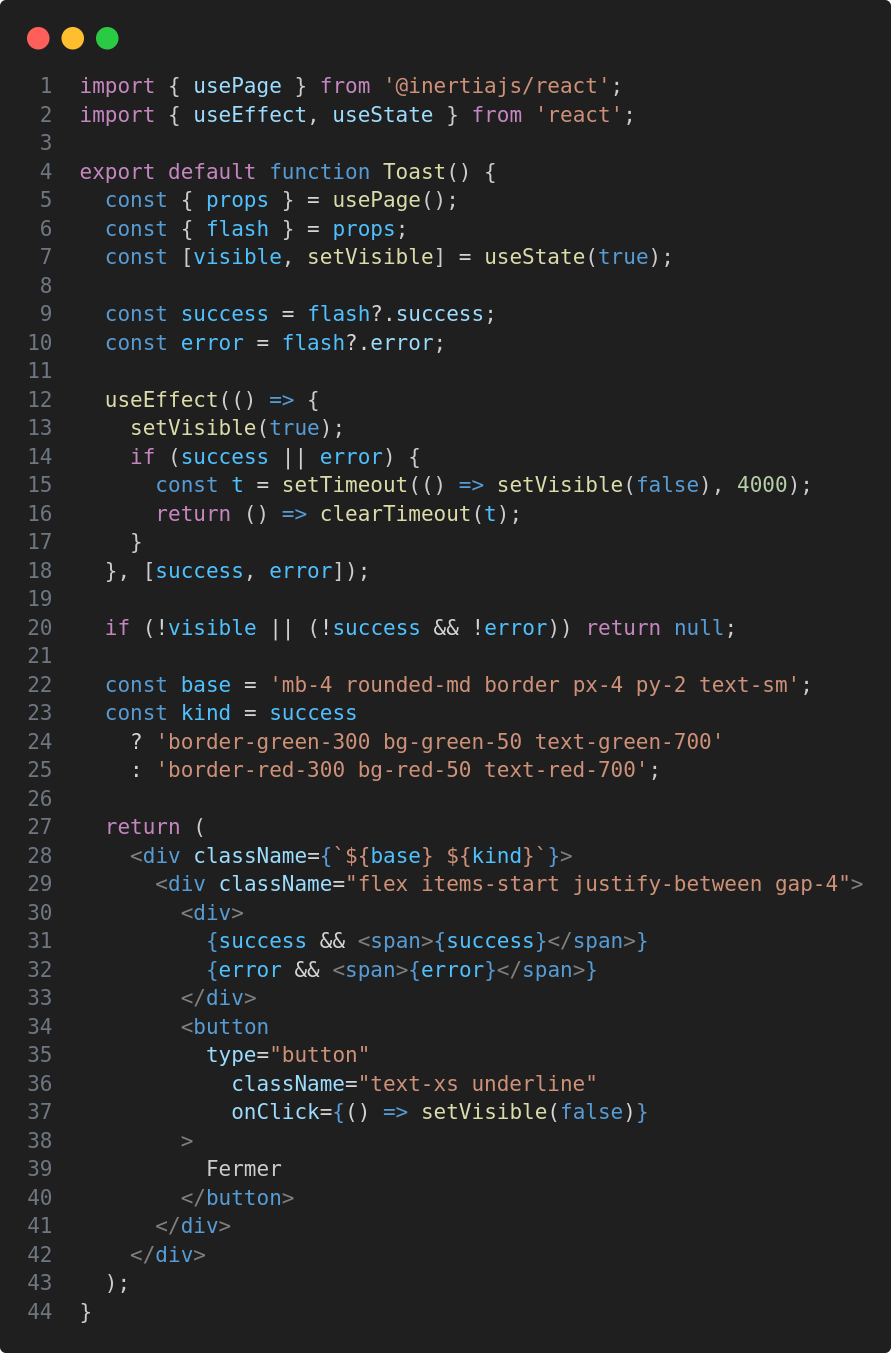
\includegraphics[width=0.5\textwidth]{figures-C1/posts_toast.png}    
    \captionsetup{singlelinecheck=true}   
    \caption{\texttt{Layouts/Toast.jsx}}
    \label{fig:posts_toast}
\end{wrapfigure}
Ce composant récupère les messages flash (success / error) envoyés par Laravel via Inertia et les affiche. Il montre le message, le cache automatiquement après 4 secondes ou immédiatement si on clique sur "Fermer". S’il n’y a rien à afficher, il ne rend rien.

Maintenant, il faut faire parvenir la variable \texttt{success} et \texttt{error} via notre \\ \texttt{PostsController} \footnote{\texttt{app/Http/Controller/PostsController.php}, de rien pour ça.}. Ajoutez-y donc ceci :

\begin{figure}[!h]
    \hspace{1cm}
    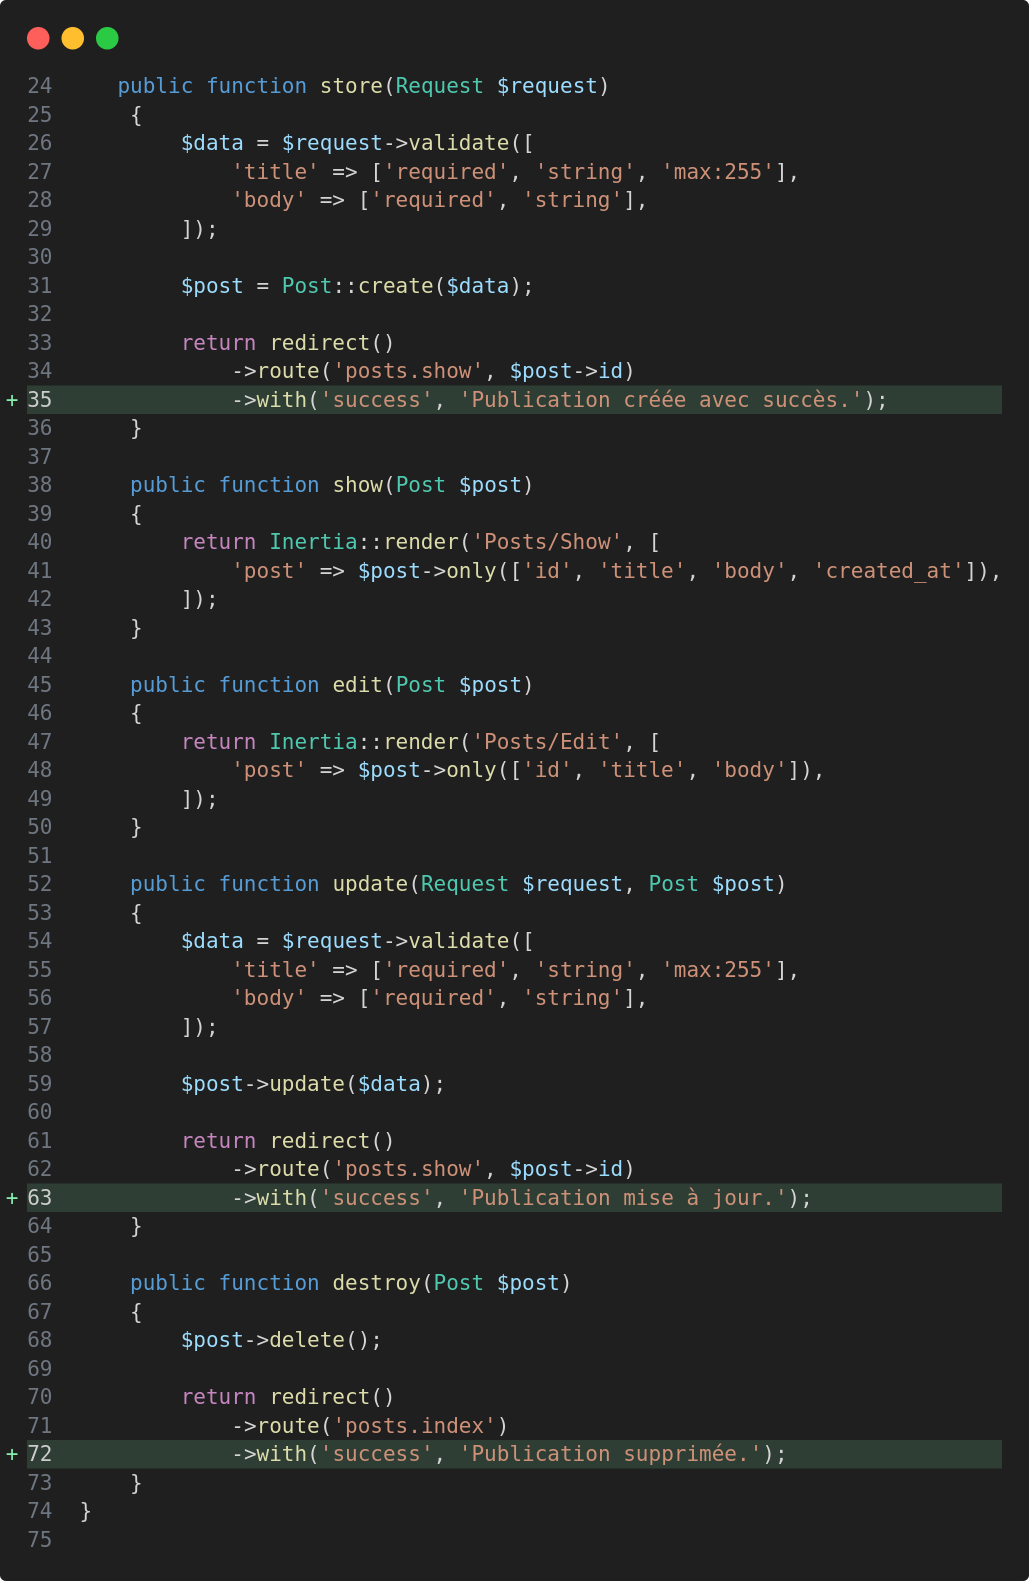
\includegraphics[width=0.3\textwidth]{figures-C1/postscontroller_toast.png}
    \label{fig:postscontroller_toast}
    \captionsetup{
    justification=raggedright,
    singlelinecheck=false
    }
    \caption{\texttt{PostsController.php}}
\end{figure}

\newpage

\begin{wrapfigure}[6]{r}{0.43\textwidth}
    \vspace{-0.5cm}
    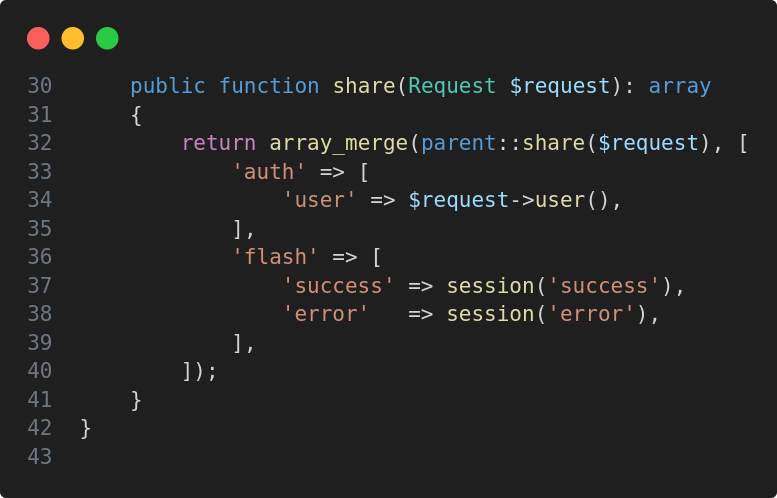
\includegraphics[width=0.43\textwidth]{figures-C1/middleware_handleinertia.png}    
    \captionsetup{singlelinecheck=false}   
    \caption{\texttt{HandleInertiaRequest.php}}
    \label{fig:middleware_toast}
\end{wrapfigure}

Avant de tester tout ça, il nous reste à permettre \inertia{} de partager ces variables. Ajoutez ceci dans le middleware \footnote{Plus de détails sur les middlewares dans la section \ref{sec:middleware}.} \\ \texttt{app/Http/Middleware/HandleInertiaRequest.php}.

Ainsi, il nous reste à ajouter les \texttt{toasts} dans notre \texttt{layout} pour les afficher à toutes les pages :

\begin{figure}[!h]
    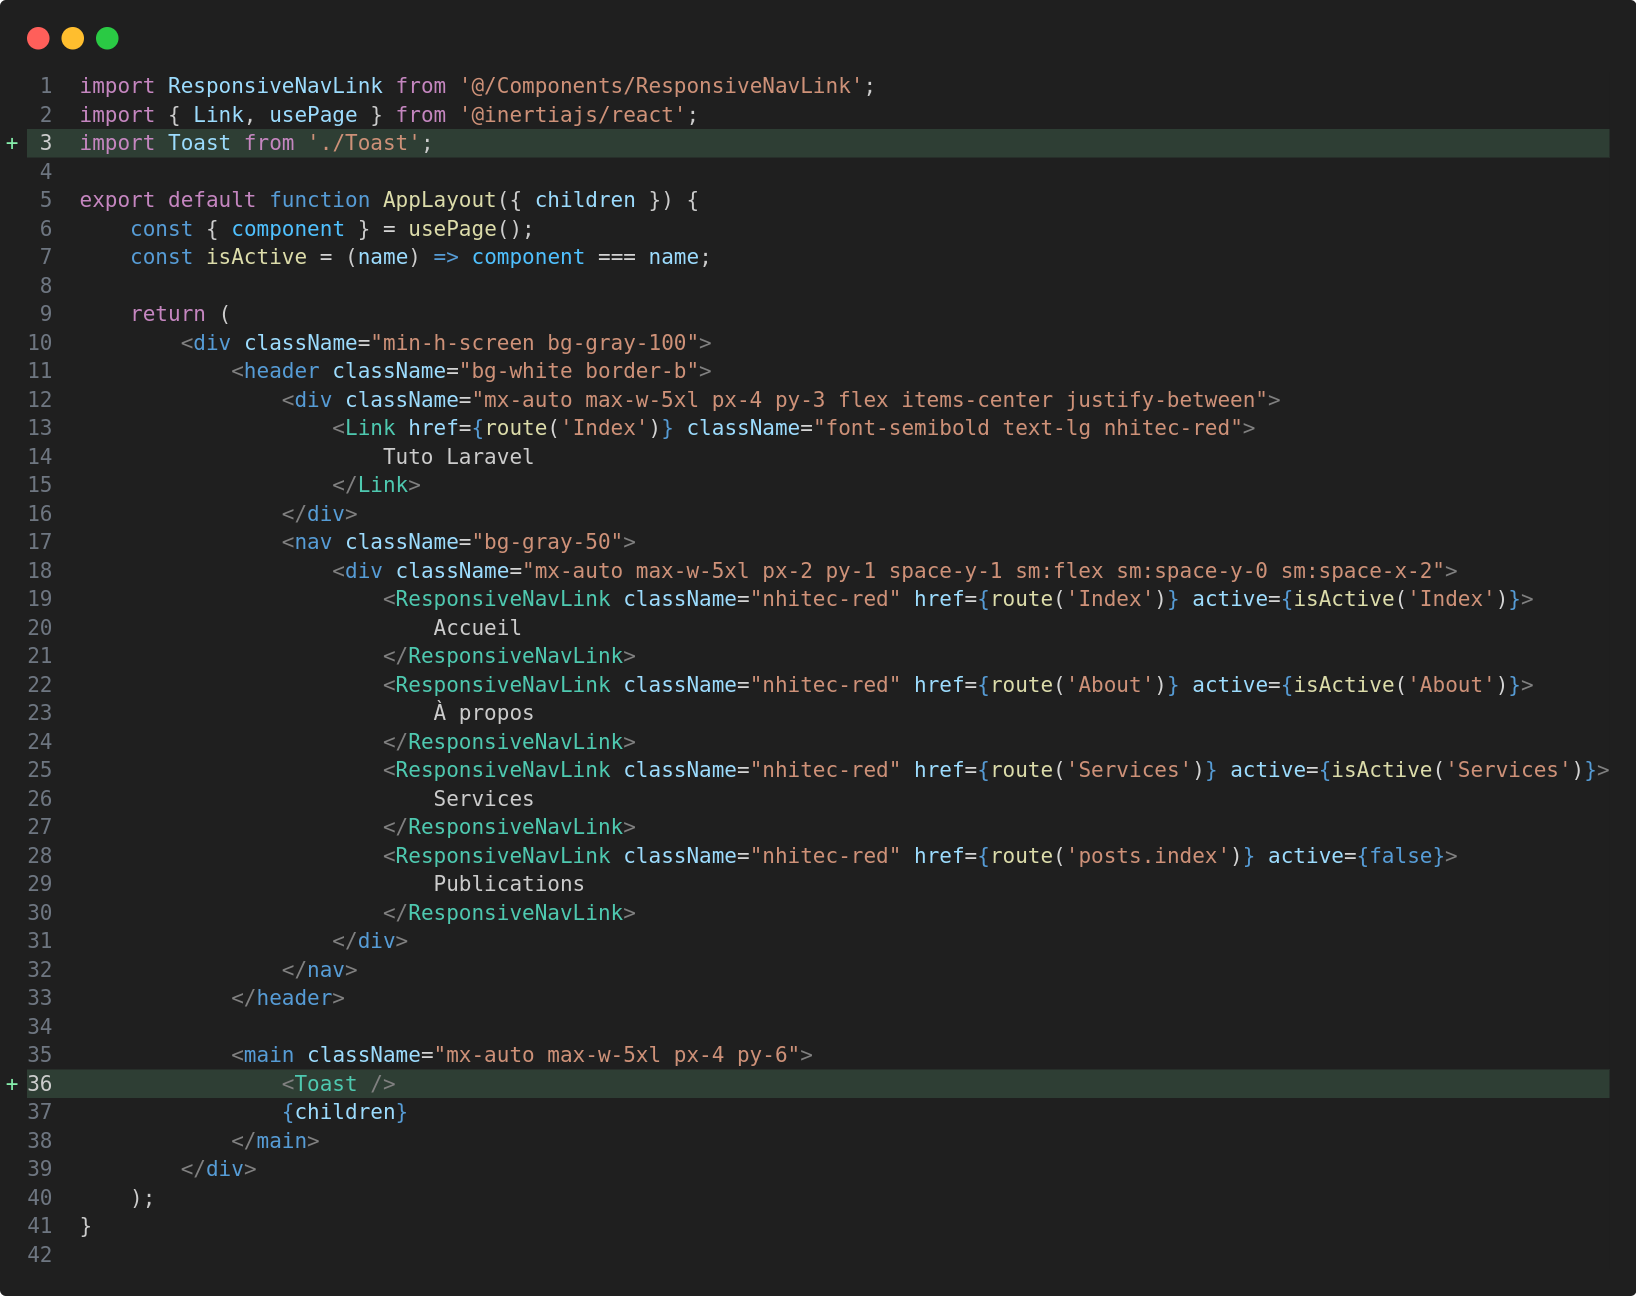
\includegraphics[width=0.5\linewidth]{figures-C1/applayout_toast.png}
    \captionsetup{
    justification=raggedright,
    singlelinecheck=false
    }
    \caption{\texttt{Layouts/AppLayout}}
    \label{fig:applayout_toast}
\end{figure}



Enfin, voici le résultat que vous devriez obtenir lorsque vous modifiez une publication.

\begin{figure}[!h]
    \centering
    \fbox{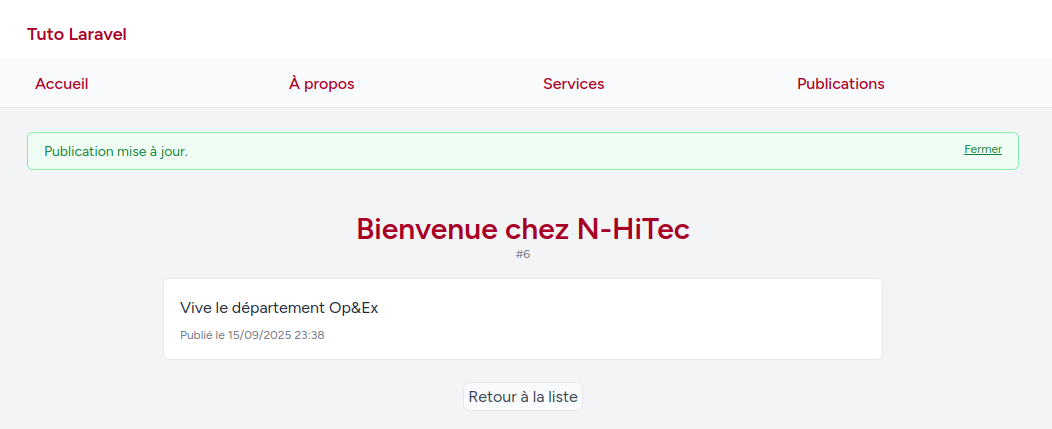
\includegraphics[width=0.8\textwidth]{figures-C1/toast_picture.png}}
    \caption{Exemple du toast de modification}
    \label{fig:toast_picture}
\end{figure}

Vous pouvez avoir l'impression que nous en avons enfin fini avec cette formation, mais \ldots il reste quelque chose qui devrait vous chiffonner : N'importe qui peut écrire et modifier les publications.

Dans la \texttt{Section~\ref{sec:auth}}, nous allons donc ajouter un système d'authentification très simple à notre site.
